Kildekoden kan ses i appendix (\ref{app:kildeKode}). 
Koden indeholder 2 hoved funktioner:
\begin{itemize}
  \item "computeDerivatives" som beregner de afledte for funktionen $f(x)$ 
  i punktet $a$, dette sker ved hjælp af python pakken SymPy, herefter returneres disse som en liste af værdier.  
  \item "intergrateTaylor" som beregner værdien af intergralet imellem to endepunkter
  og returnere værdierne for intergralet $\int_{-1}^1 P_N (x) dx$ ved specifike ordener $N$. 
\end{itemize}
Når koden køres fåes følgende værdier:
\begin{table}[H]
  \begin{center}
    \begin{tabular}{ |c|c|c|c|c|c|c| }
      \hline
        Antal led $N$ & 10 & 20 & 50 & 100 & 200 & 500 \\
      \hline
        Approximation & $1.5852$ & $1.5763$ & $1.5723$ & $1.5713$ & $1.5709$ & $1.5708$ \\
      \hline
    \end{tabular}
    \caption{Approksimationen i forhold til ordenen af taylor polynomiet}
  \end{center}
\end{table}
%\label{tab:approksimationenVsN}
Som det kan ses i tabellen sker der en mindre og mindre ændring i værdien for approksimationen når $N$ bliver større og større
I denne sammenhæng er det også intressant at kigge på fejlen imellem approksimationen $\int_{-1}^1 P_N(x) dx$ og $\frac{\pi}{2}$:
\begin{figure}[H]
  \centering
  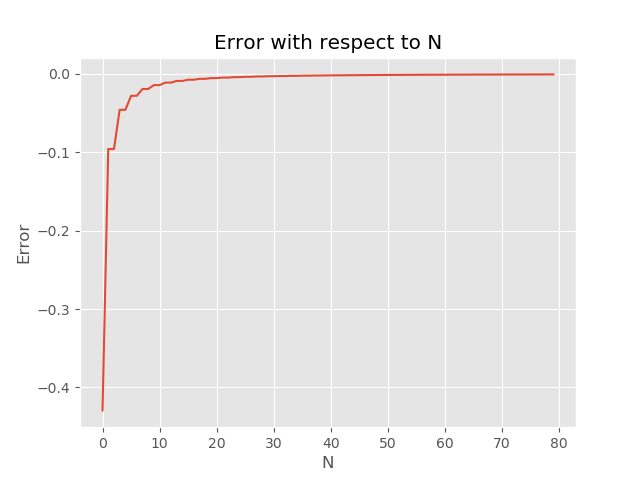
\includegraphics[width=\textwidth]{fig/img/ErrorWithRespectToN.png}
  \caption{Fejl i forhold til antalet af led $N$}
  \label{fig:FejlIForholdTilN}
\end{figure}
Som det kan ses falder fejlen hurtigt i starten når $N$ er lille, men som $N$ vokser flader fejlen ud fordi $P_{N-1}(x) \approx P_{N}(x)$ når $N \rightarrow \infty$.